% !TeX spellcheck = en_US
\documentclass[letterpaper,12pt,twoside]{report}
\usepackage{fancyhdr}
\usepackage{fullpage}
\usepackage{tikz}
\usepackage{amsmath}

\begin{document}
	\pagestyle{fancy}
	\fancyhf{}
	\fancyhead[L]{Day 5}
	\fancyhead[R]{\textit{The Calendar Project}}
	\fancyfoot[L]{Citations Involved: 1, 2, 3}
	
	% Problem
	\paragraph{Problem}
	\begin{quote}
	\textsf{Consider the parabola with equation $y = x^2$ and the rectangle with vertices $(1,0)$, $(1,1)$, $(-1,1)$, and $(-1, 0)$. Find the area of the parabolic segment (shaded) and compare its area with that of the rectangle.}
	\end{quote}
	
	% Graphics
	\begin{minipage}{.45\linewidth}
	\begin{center}
		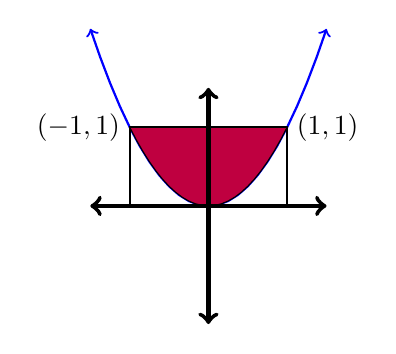
\begin{tikzpicture}
		
		\draw [<->][blue, thick, domain=-1.5:1.5] plot (\x, {\x*\x});
		\draw [thick] (-1,0) -- (-1, 1) -- (1, 1) -- (1, 0);
		\draw[fill=purple,domain=-1:1] (-1,1) -- plot ({\x},{\x*\x}) -- (1,1) -- cycle;
		
		\draw [<->][ultra thick] (-1.5,0) -- (1.5,0);
		\draw [<->][ultra thick] (0,1.5) -- (0,-1.5);
		
		\node[left] at (-1,1) {$(-1,1)$};
		\node[right] at (1,1) {$(1,1)$};
		\end{tikzpicture}
	\end{center}
\end{minipage}
\begin{minipage}{.45\linewidth}
	\begin{center}
		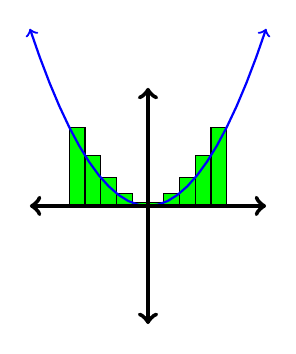
\begin{tikzpicture}
			\draw[fill=green] (-1,1) -- (-0.8,1) -- (-0.8,0) -- (-1,0) -- cycle;
			\draw[fill=green] (-0.8,0.64) -- (-0.6,0.64) -- (-0.6,0) -- (-0.8,0) -- cycle;
			\draw[fill=green] (-0.6,0.36) -- (-0.4,0.36) -- (-0.4,0) -- (-0.6,0) -- cycle;
			\draw[fill=green] (-0.4,0.16) -- (-0.2,0.16) -- (-0.2,0) -- (-0.4,0) -- cycle;
			\draw[fill=green] (-0.2,0.04) -- (0,0.04) -- (0,0) -- (-0.2,0) -- cycle;
			\draw[fill=green] (0,0.04) -- (0.2,0.04) -- (0.2,0) -- (0,0) -- cycle;
			\draw[fill=green] (0.4,0.16) -- (0.2,0.16) -- (0.2,0) -- (0.4,0) -- cycle;
			\draw[fill=green] (0.6,0.36) -- (0.4,0.36) -- (0.4,0) -- (0.6,0) -- cycle;
			\draw[fill=green] (0.8,0.64) -- (0.6,0.64) -- (0.6,0) -- (0.8,0) -- cycle;
			\draw[fill=green] (1,1) -- (0.8,1) -- (0.8,0) -- (1,0) -- cycle;
			\draw[<->][blue,thick,domain=-1.5:1.5] plot (\x,{\x*\x});
			
			\draw [<->][ultra thick] (-1.5,0) -- (1.5,0);
			\draw [<->][ultra thick] (0,1.5) -- (0,-1.5);
		\end{tikzpicture}
	\end{center}
\end{minipage}
	
	\paragraph{Introduction to Derivatives}
	\begin{quotation}
	Google defines the Derivative as ``an expression representing the rate of change of a function with respect to an independent variable.'' In a graph of $y=f(x)$ on the coordinate plane, a Derivative refers to the instantaneous slope with respect to $x$. 
\end{quotation}

	\paragraph{Introduction to Integral Calculus}
	\begin{quotation}
		This problem is a typical application of the classic ``area under a curve'' problem that introduces many students to Integral Calculus.
		
		Consider the area of the {\color{green} green} rectangles above as an approximation of the area under the parabola $y=x^2$ from $x=-1$ to $x=1$. This is an application of the Riemann Sum. Let the width of each rectangle be $\Delta x$; since the area formula for a rectangle is $wl$ where $w$ is its width and $l$ is its length, the area of one such rectangle can be expressed as $x^2\Delta x$ where $x$ represents its horizontal displacement from the $y$-axis. As such, the approximate area under $y=x^2$ bounded by the $y$-axis and $x=g$ can be expressed as $\sum\limits_{n=1}^{\frac{|g|}{\Delta x}}(n\Delta x)^2\Delta x=\sum\limits_{n=1}^{\frac{|g|}{\Delta x}}n^2(\Delta x)^3$ where $g$ is a multiple of $\Delta x$. To represent the exact solution, $\Delta x$ must be infinitesimal; thus the exact area is $\lim\limits_{\Delta x \rightarrow 0}\sum\limits_{n=1}^{\frac{|g|}{\Delta x}}n^2(\Delta x)^3$.
	\end{quotation}
	
	% Reasoning
	\paragraph{Reasoning}
	\begin{quotation}
	
	The complement of the condition that \textit{``at least 1 six appears''} is that no six appears, which has a probability of $\frac{\textrm{\small{favorable}}}{\textrm{\small{all possible}}} = \frac{5}{6}$ for 1 roll (1). Since it is given that the die is tossed 6 times, and since this negated condition requires \textbf{all} rolls (not just one) to not be six, the cumulative probability for this negated condition is $(\frac{5}{6})^6 = \frac{5^6}{6^6} = \frac{15625}{46656}$ (3). This result's complement, the solution to the problem, is $1-\frac{15625}{46656} = \boxed{\frac{31031}{46656} \approx 0.665}$ (2) 
	
	\end{quotation}
	
	\paragraph{External References}
	
	\begin{enumerate}
		\item Textbook Ch. 13, Pg. 878: Theoretical Probability
		\item Textbook Ch. 13, Pg. 879: Complement
		\item Textbook Ch. 13, Pg. 887: Probability of Independent Events
	\end{enumerate}

\end{document}